\documentclass[10pt,letter]{article}
\usepackage{amsmath}
\usepackage{amssymb}
\usepackage{graphicx}
\usepackage{setspace}
%\onehalfspacing
\usepackage{fullpage}
\usepackage{verbatimbox}
\begin{document}

\title{Problem Set 1 - CS 7641 - Completed}
\author{Magahet Mendiola}
%\date{Submit by Feb 20, 2014}
\maketitle

%Instructions: This problem set is not a part of your final grade. Solve atleast 3 of these problems and submit your solutions on t-square. We will not grade them, but we will provide solutions at the end of the deadline for you to compare your answers. If your final score falls very close to the switchover point to the next higher grade, we will grade your submission of this problem set for input into determining your final grade.

\paragraph{2} Design a two-input perceptron that implements the boolean function $A \land \lnot B$. Design a two-layer network of perceptrons that implements $A \oplus B$ ($\oplus$ is XOR).

\paragraph{2 - Answer}

Below is a diagram of an XOR ANN:

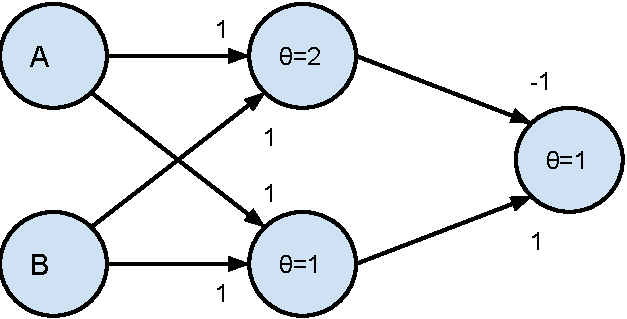
\includegraphics[width=3in]{xor_ann.pdf}

The top hidden node activates when both A and B are 1, which prevents the output node from activating due to the negative weight from this node.

The bottom node activates when either or both A and B are 1, which activates the output node if not prevented from doing so by the top hidden node.


\paragraph{4} Explain how you can use Decision Trees to perform regression? Show that when the error function is squared error, then the expected value at any leaf is the mean. Take the Boston Housing dataset (https://archive.ics.uci.edu/ml/datasets/Housing) and use Decision Trees to perform regression. 

\paragraph{4 - Answer}

To perform regression using a decision tree we need an algorithm with these components:

\begin{description}
    \item[Splitting Criteria] This is similar to selecting attributes or value thresholds with the highest information gain. In the case of continuous output values, we could evaluate splits based on the mean squared error of the two resulting subsets of instances. Attributes and value thresholds would be selected by minimizing this error function.
    \item [Leaf Valuation Method] If we split nodes based on mean squared error, then the value at any given node is the mean of all the output values under that node. This can be seen in the derivation shown in the lecture on loss error functions. In simplistic terms, the constant that results in the derivative of the loss function equaling zero is the mean of the values.
    \item [Stopping Criteria] One way to determine when to stop creating new branches could be when a node reaches some minimum number of instances.
\end{description}

Using Weka's M5P algorithm, which is based on the M5 algorithm, we can set the parameters to build a regression tree instead of a Model tree. Figure~\ref{regression-tree}, shows the resulting tree and performance metrics. A smaller tree was produced by setting the minimum number of instances in a leaf to 100.

\scriptsize
\begin{verbbox}
LSTAT <= 9.725 : 
|   RM <= 6.941 : 
|   |   DIS <= 3.325 : 27.3677 (30/103.003%)
|   |   DIS >  3.325 : 
|   |   |   RM <= 6.545 : 23.848 (72/25.571%)
|   |   |   RM >  6.545 : 26.7514 (40/35.115%)
|   RM >  6.941 : 36.0038 (70/84.479%)
LSTAT >  9.725 : 
|   LSTAT <= 15 : 
|   |   DIS <= 4.428 : 
|   |   |   TAX <= 300 : 21.8909 (21/34.287%)
|   |   |   TAX >  300 : 20.3158 (79/32.793%)
|   |   DIS >  4.428 : 19.7139 (32/19.206%)
|   LSTAT >  15 : 
|   |   CRIM <= 5.769 : 17.0209 (83/37.146%)
|   |   CRIM >  5.769 : 13.3508 (79/40.185%)


Correlation coefficient                  0.8374
Mean absolute error                      3.6274
Root mean squared error                  4.9421
Relative absolute error                 56.3733 %
Root relative squared error             55.4895 %

\end{verbbox}
\normalsize

\begin{figure}[!htbp]
    \theverbbox
    \centering
    \caption{Regression Tree - Housing Data\label{regression-tree}}
\end{figure}

From this we see that splitting first on the attribute LSTAT (\% lower status of the population) at 9.725 resulted in the lowest error for instances on either side of the split. It's interesting that LSTAT is again the best discriminator at value 15. The lowest home value occurred when LSTAT was over 15 and the crime rate was over 5.769. This makes intuitive sense. Conversely, the lowest LSTAT and largest average number of rooms resulted in the highest home value.




\paragraph{5} Suggest a lazy version of the eager decision tree learning algorithm ID3. What are the advantages and disadvantages of your lazy algorithm compared to the original eager algorithm?

\paragraph{5 - Answer}

The algorithm would build a new tree on each query in the same way as ID3, with a few exceptions:

\begin{enumerate}
    \item Find the attribute that maximizes information gain on current training set. Only consider attributes that are not missing from the query.
    \item Reduce the current training set to those instances that match the query's value for the selected attribute.
    \item Repeat steps 1 and 2 until all the instances in the current training set have the same class or the query has no remaining attributes to evaluate.
    \item Return either the unanimous class or the most common class from the remaining training instances.
\end{enumerate}

The eager version of ID3 requires that queries have all the attributes found in the training set; or at least enough to transverse to a leaf node. The lazy version would be more robust in this case. A query with even a single attribute would be able to return a class.

The lazy decision tree query time could be as little as doing lookup of instances that match a single attribute value, or as much as it would take to build a full tree down a single branch. In either case, it should not be more than building the full tree, as with the eager version. However, it would need to perform the full training process on each query, making it eventually less efficient for a large number of queries.

The lazy tree may also be more accurate, as decision nodes are built on only the subset of attributes that occur in the query. This would focus the information gain measurements to only the relevant instances in the training set.


\end{document}
